\chapter{Аналитическая часть}

\section{Анализ предметной области}

Проведение кубка мира по шахматам регламентируется международной шахматной федерацией (ФИДЕ)~\cite{fidewc}.
В турнире принимают участие 206 человек~\cite{fidewc}.
Соревнование состоит из восьми раундов~\cite{fidewc}.
Количество участников в каждом раунде представлено в таблице~\ref{fidewcrounds}.
\begin{center}
	\begin{threeparttable}
		\captionsetup{justification=raggedright,singlelinecheck=off}
		\caption{\label{fidewcrounds}Количество участников в каждом раунде кубка мира по шахматам}
		\centering
		\begin{tabular}{|c|c|}
			\hline
			Раунд & Количество участников \\
			\hline
			Раунд 1 & 156 \\
			\hline
			Раунд 2 & \specialcell{128\\(78 победителей раунда 1 и\\50 игроков с самым высоким рейтингом)} \\
			\hline
			Раунд 3 & 64 \\
			\hline
			Раунд 4 & 32 \\
			\hline
			Раунд 5 & 16 \\
			\hline
			Раунд 6 & 8 \\
			\hline
			Раунд 7 & 4 \\
			\hline
			Раунд 8, матч за третье место & 2 \\
			\hline
			Раунд 8, финал & 2 \\
			\hline
		\end{tabular}
	\end{threeparttable}
\end{center}

Турнир проводится по нокаут-системе~\cite{fidewc}.
В каждом раунде матч между двумя шахматистами состоит из двух партий с временным контроллем ФИДЕ: участникам дается 90 минут на первые 40 ходов, затем~--- 30 минут на оставшуюся часть игры с увеличением времени на 30 секунд после каждого хода, начиная с первого хода~\cite{fidewc}.
Игрок, набравший по прошествию двух партий большее число очков, чем его соперник, становится победителем матча и переходит на следующий раунд~\cite{fidewc}.

Если количество очков игроков матча одинаковы, проводится тай-брейк: две партии по 25 минут на каждого игрока с увеличением времени на 10 секунд после каждого хода, начиная с первого~\cite{fidewc}.

Если в результате первого тай-брейка участники снова оказались в состоянии ничьи, проводятся две партии по 10 минут на каждого игрока с увеличением времени на 10 секунд после каждого хода, начиная с первого~\cite{fidewc}.

Если в результате второго тай-брейка участники снова оказались в состоянии ничьи, проводятся две партии по 5 минут на каждого игрока с увеличением времени на 3 секунды после каждого хода, начиная с первого~\cite{fidewc}.

Если в результате третьего тай-брейка участники снова оказались в состоянии ничьи, проводится одна партия~--- 3 минуты на каждого игрока с увеличением времени на 2 секунды после каждого хода, начиная с первого~\cite{fidewc}.

Если в результате четвертого тай-брейка участники снова оказались в состоянии ничьи, проводится одна партия~--- 3 минуты на каждого игрока с увеличением времени на 2 секунды после каждого хода, начиная с первого, со сменой цветов фигур~\cite{fidewc}.

Если в результате пятого тай-брейка участники снова оказались в состоянии ничьи, то партия повторяется вновь до тех пор, пока не будет выявлен победитель~\cite{fidewc}.

После каждой сыгранной партии меняется рейтинг шахматистов, который формируется международной шахматной федерацией на основе метода расчета Эло~\cite{fideraiting, elo}.
Перед вычислением нового рейтинга определяется вероятность $PD$ достижения игроком результата в каждой партии по таблице~\ref{pd}.
\begin{center}
	\begin{threeparttable}
		\captionsetup{justification=raggedright,singlelinecheck=off}
		\caption{\label{pd}Таблица преобразования разницы в рейтинге D в вероятность достижения
			результата PD игроком с более высоким рейтингом H и игроком с более низким
			рейтингом L, соответственно}
		\centering
		\begin{tabular}{|c|c|c|c|c|c|c|c|c|c|c|c|}
			\hline
			D & \multicolumn{2}{|c|}{PD} & D & \multicolumn{2}{|c|}{PD} & D & \multicolumn{2}{|c|}{PD} & D & \multicolumn{2}{|c|}{PD} \\
			\hline
			& H & L && H & L && H & L && H & L\\
			\hline
			0--3&.50&.50&92--98&.63&.37&198--206&.76&.24&345--357&.89&.11\\
			\hline
			4--10&.51&.49&99--106&.64&.36&207--215&.77&.23&358--374&.90&.10\\
			\hline
			11--17&.52&.48&107--113&.65&.35&216--225&.78&.22&375--391&.91&.09\\
			\hline
			18--25&.53&.47&114--121&.66&.34&226--235&.79&.21&392--411&.92&.08\\
			\hline
			26--32&.54&.46&122--129&.67&.33&236--245&.80&.20&412--432&.93&.07\\
			\hline
			33--39&.55&.45&130--137&.68&.32&246--256&.81&.19&433--456&.94&.06\\
			\hline
			40--46&.56&.44&138--145&.69&.31&257--267&.82&.18&457--484&.95&.05\\
			\hline
			47--53&.57&.43&146--153&.70&.30&268--278&.83&.17&485--517&.96&.04\\
			\hline
			54--61&.58&.42&154--162&.71&.29&279--290&.84&.16&518--559&.97&.03\\
			\hline
			62--68&.59&.41&163--170&.72&.28&291--302&.85&.15&560--619&.98&.02\\
			\hline
			69--76&.60&.40&171--179&.73&.27&303--315&.86&.14&620--735&.99&.01\\
			\hline
			77--83&.61&.39&180--188&.74&.26&316--328&.87&.13&>735&1.0&.00\\
			\hline
			84--91&.62&.38&189--197&.75&.25&329--344&.88&.12&&&\\
			\hline
		\end{tabular}
	\end{threeparttable}
\end{center}

После получения значения $PD$ для конкретного игрока вычисляется величина:
\begin{equation}\label{dr}
	\Delta{R} = Res - PD,
\end{equation}
где $Res$~--- результат партии (1~--- выигрыш, 0.5~--- ничья, 0~--- проигрыш)~\cite{fideraiting}.

Изменение рейтинга игрока вычисляется по формуле:
\begin{equation}\label{raitingdelta}
	\Delta{S} = \Sigma{\Delta{R}} \cdot K,
\end{equation}
где $\Sigma{\Delta{R}}$~--- сумма всех $\Delta{R}$ для турнира или рейтингового периода,\\
\text{~~~~~~}$K = 20,$ если рейтинг игрока не превышает 2400,\\
\text{~~~~~~}$K = 10,$ если рейтинг игрока превышает 2400~\cite{fideraiting}.

Если количество партий $n$ для игрока в любом списке за рейтинговый период, умноженное на $K$ (как определено выше), превышает 700, то в качестве $K$ выбирается такое наибольшее целое число, что произведение числа $K$ на $n$ не превышает 700~\cite{fideraiting}.

Во время проведения кубка мира по шахматам возможен прием ставок~--- подкрепленных деньгами прогнозов на исходы каких-либо событий~\cite{bet}.
Для каждого условия устанавливается коэффициент, определяющий чистую прибыль участников при выигрыше спора~\cite{bet}.

Существуют следующие виды ставок~\cite{bet}:
\begin{itemize}
	\item главная линия (исход партии~--- победа первого участника, ничья и т.д.),
	\item тоталы (количество свершенных событий в течение партии, матча, раунда или турнира),
	\item форы (с каким отрывом выиграет участник),
	\item экспрессы (объединение нескольких исходов в одну ставку),
	\item системы (объединение экспрессов в одну ставку).
\end{itemize}

В шахматных турнирах форы быть не может, поскольку во время партии не ведется счет очков, поэтому вводится понятие нулевой форы, при которой ставка делается на том, что один из участников, как минимум, не проиграет~\cite{chessbet}.

При объединении исходов в экспресс их коэффициенты перемножаются, при этом для выигрыша необходимо, чтобы все поставленные условия были выполнены~\cite{bet}.

Системы имеют размерность~--- пару натуральных чисел, определяющих количество исходов, из которых составляются экспрессы, и количество событий в каждом из экспрессов~\cite{bet}.
Выигранная денежная сумма вычисляется на основе коэффициентов свершенных экспрессов~\cite{bet}.

\section[Анализ существующих решений и требования к разрабатываемым базе данных и приложению]{Анализ существующих решений и требования к\\разрабатываемым базе данных и приложению}

В таблице~\ref{chessdbs} представлен сравнительный анализ существующих аналогов базы данных для хранения информации о сыгранных шахматных партиях.
\begin{center}
	\begin{threeparttable}
		\captionsetup{justification=raggedright,singlelinecheck=off}
		\caption{\label{chessdbs}Сравнительный анализ существующих аналогов}
		\centering
		\begin{tabular}{|c|c|c|c|c|}
			\hline
			& Тип & Открытый && Возможность\\
			Название & программного & исходный &  Бесплатный & делать\\
			& обеспечения & код && ставки\\
			\hline
			Scid~\cite{scid} & Десктопное & + & + & -\\
			\hline
			ChessGames~\cite{chessgamescom} & Веб-сайт & - & + & -\\
			\hline
			365Chess~\cite{365chess} & Веб-сайт & - & + & -\\
			\hline
			FicsGames~\cite{fics} & Веб-сайт & - & + & -\\
			\hline
		\end{tabular}
	\end{threeparttable}
\end{center}

Требования к разрабатываемым базе данных и приложению:
\begin{itemize}
	\item база данных должна быть разработана для хранения информации о сыгранных в кубке мира шахматных партиях, выполненных в них ходах, игроках, судьях, ставках и пользователях системы;
	\item приложение должно быть разработано для работы с информацией, хранящейся в базе данных;
	\item пользователю должна быть предоставлена возможность добавлять, удалять и получать информацию о сыгранных шахматных партиях, выполненных в них ходах, игроках, судьях, ставках и пользователях системы;
	\item в приложении должно быть предусмотрено логирование на всех уровнях;
	\item приложение должно иметь два кэша: для передачи запросов от приложения в систему управления базой данных и для передачи информации от бэкенда во фронтенд.
\end{itemize}

\section{Системы управления базами данных}

Система управления базой данных (СУБД)~--- программное обеспечение, предоставляющее создание, обновление, хранение и поиск информации в базе данных~\cite{db}.
СУБД имеет следующие функции~\cite{db}:
\begin{itemize}
	\item предоставление средств определения данных в виде исходной формы и преобразование этих определений в соответствующую объектную форму;
	\item обработка запросов пользователя на выборку, изменение, добавление или удаление данных;
	\item оптимизация способа выполнения каждого из запросов;
	\item защита и поддержка целостности данных;
	\item восстановление данных;
	\item поддержка параллельности;
	\item выполнение функций с максимально возможной эффективностью.
\end{itemize}

По направленности системы управления базами данных классифицируются следующим образом~\cite{dbmsu}:
\begin{itemize}
	\item универсальные,
	\item специализированные.
\end{itemize}

Универсальные СУБД не ориентированы на какую-либо предметную область~\cite{dbmsu}.
Каждая система такого рода является универсальной и реализует функционально избыточное множество операций над данными~\cite{dbmsu}.

Специализированные СУБД предназначены для конкретных классов задач, которые не могут быть оптимально решены с помощью универсальных систем~\cite{dbmsu}.

По способу доступа системы управления базами данных делятся на~\cite{dbmsu}:
\begin{itemize}
	\item клиент-серверные,
	\item файл-серверные,
	\item встраиваемые.
\end{itemize}

В файл-серверных СУБД база данных хранится на специализированном сервере, а СУБД запускается на стороне клиента~\cite{dbmsu}.
Как правило, такая архитектура используется внутри локальной сети~\cite{dbmsu}.
Многопользовательская синхронизация осуществляется на уровне сервера, что влечёт многочисленные блокировки файлов~\cite{dbmsu}.
Сервер только хранит данные, и не обрабатывает их, поэтому ответ от такого файл-сервера будет в виде блока данных для каждого запроса, что влечет за собой высокую нагрузку на сеть при большом числе клиентов~\cite{dbmsu}.
Файл-серверные СУБД считаются устаревшими и пригодны для работы при малом количестве клиентов (до нескольких десятков)~\cite{dbmsu}.

В клиент-серверных СУБД все основные компоненты выполняются на отдельном сервере, содержащем базу данных~\cite{dbmsu}.
На клиенте находится интерфейсная часть СУБД и выполняется код приложения~\cite{dbmsu}.
Достоинством клиент-серверной архитектуры является оптимизация на стороне клиента: всю работу с базой данных осуществляет сервер, по сети передаётся только обработанный ответ~\cite{dbmsu}.
Недостатком клиент-серверной архитектуры является зависимость клиентов от сервера, так как, в случае неисправной работы последнего, теряется возможность получения доступа к базе данных~\cite{dbmsu}.

Встраиваемые СУБД подразумевают хранение базы данных в оперативной памяти клиента во время работы приложения~\cite{dbmsu}.
Как правило, встраиваемые СУБД представляют собой библиотеки, функции которой используются в коде программы~\cite{dbmsu}.
Основным недостатком встраиваемых СУБД является незащищенность базы данных от программы клиента~\cite{dbmsu}.

\section[Описание сущностей проектируемой базы данных]{Описание сущностей проектируемой\\базы данных}

На рисунке~\ref{er} представлена ER-диаграмма сущностей проектируемой базы данных в нотации Чена.
\begin{figure}[H]
	\centering
	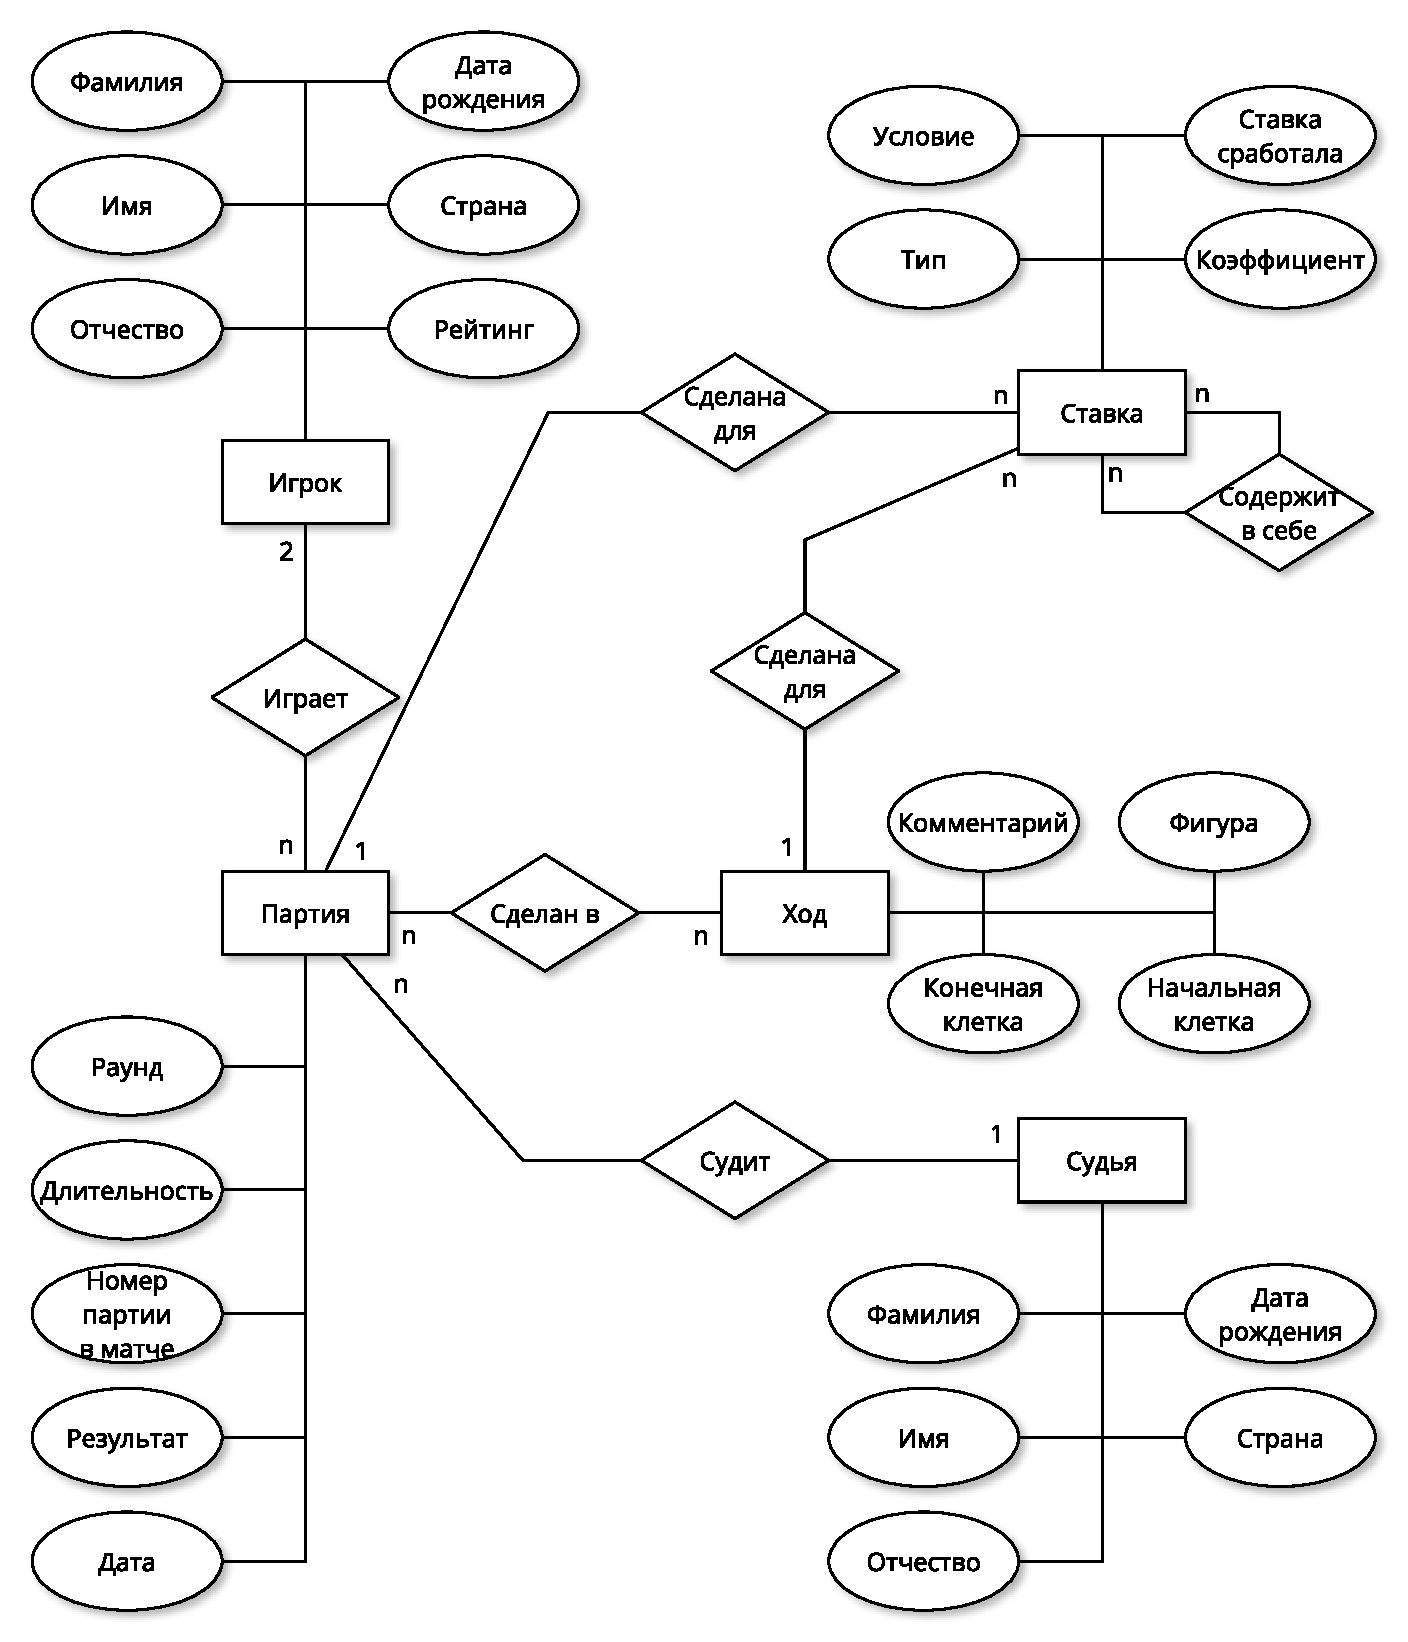
\includegraphics[width=\columnwidth]{er}
	\caption{ER-диаграмма сущностей проектируемой базы данных}
	\label{er}
\end{figure}

\section[Описание пользователей проектируемого приложения]{Описание пользователей\\проектируемого приложения}

На рисунке~\ref{usecase} представлена диаграмма вариантов использования проектируемого приложения.
\begin{figure}[H]
	\centering
	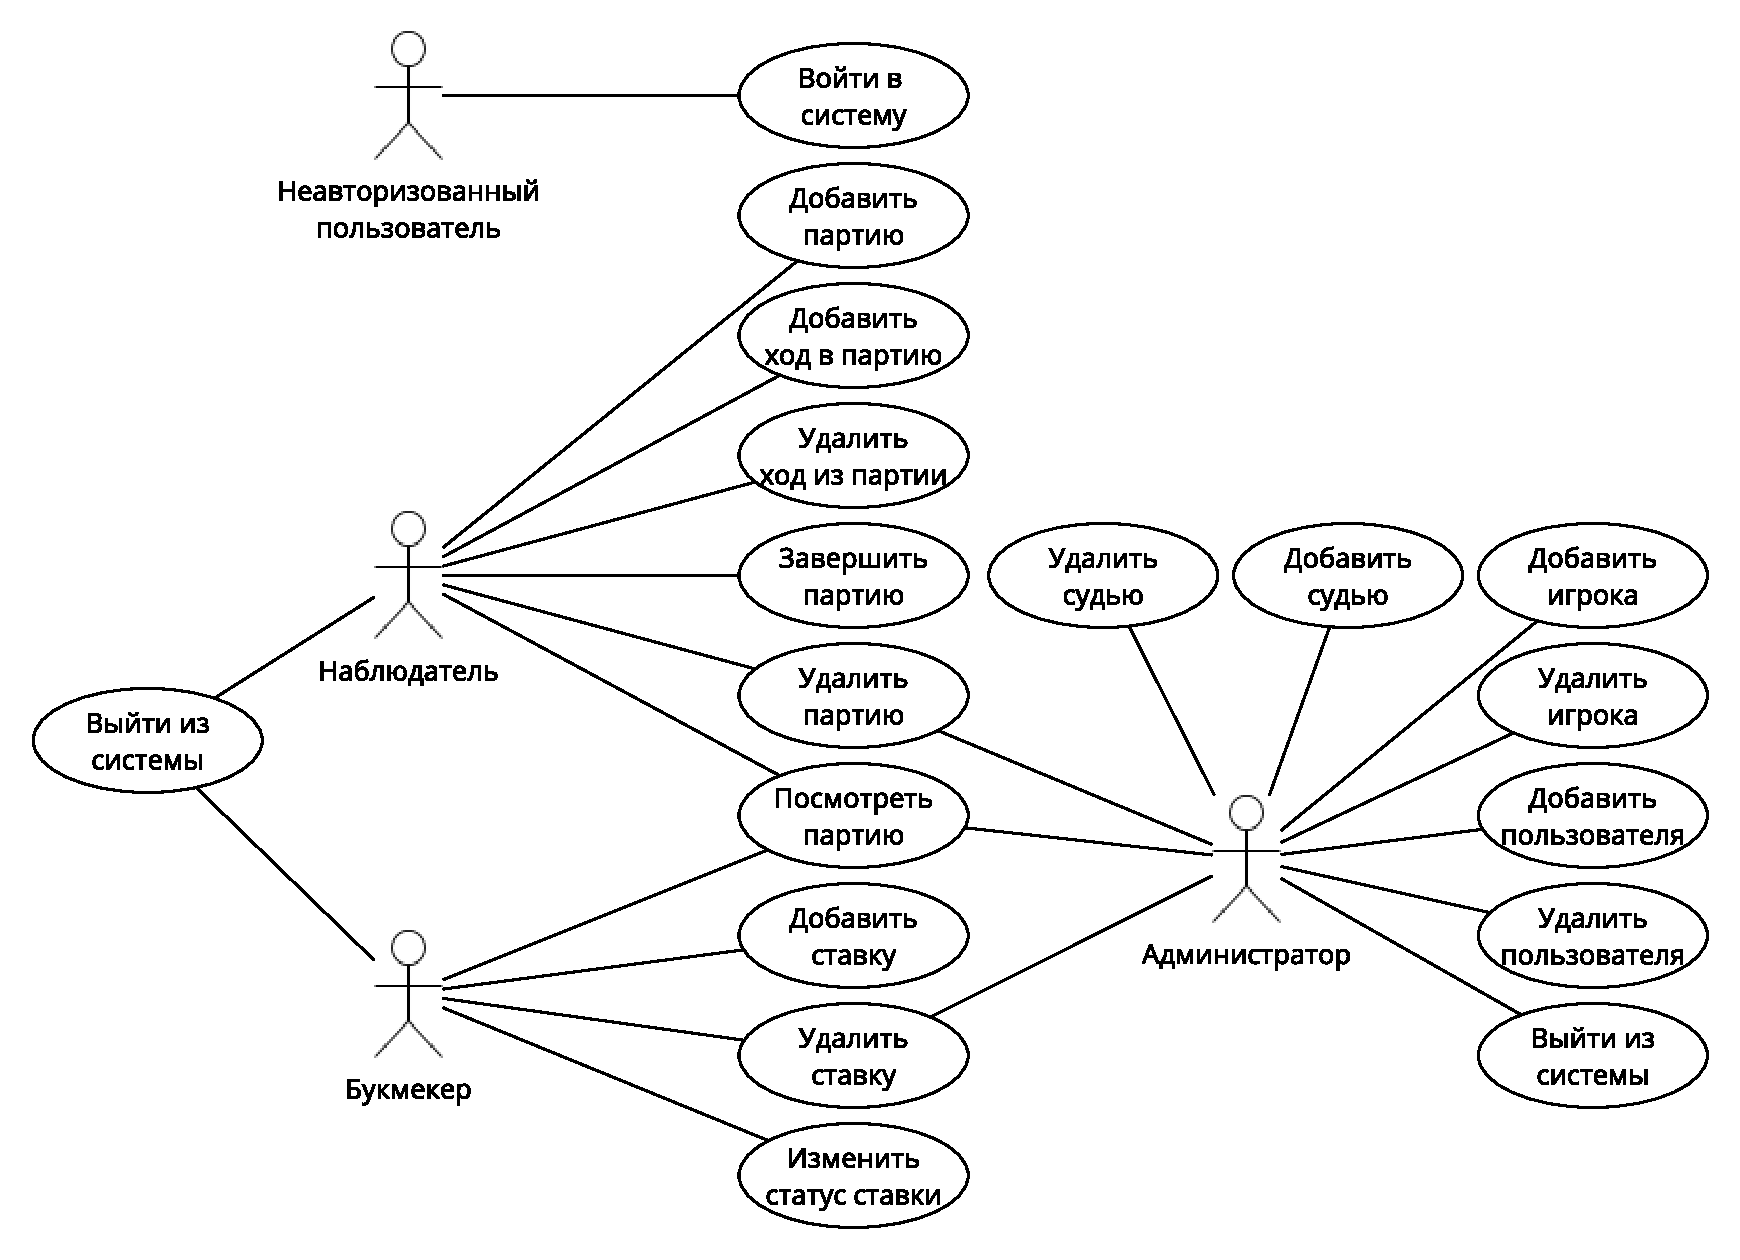
\includegraphics[width=\columnwidth]{usecase}
	\caption{Диаграмма вариантов использования проектируемого приложения}
	\label{usecase}
\end{figure}

Неавторизованный пользователь не имеет доступа к информации, хранящейся в базе данных, поэтому для получения соответствующих прав ему необходимо войти в систему.

Судья~--- человек, следящий за проведением шахматных партий. Судье дана возможность добавлять и удалять партии и ходы, выполненные в них.

Букмекер~--- лицо, осуществляющее прием ставок. Букмекер имеет возможность добавлять, удалять и редактировать информацию о спорах.

Администратор~--- лицо, ответственное за добавление и удаление пользователей системы и игроков из базы данных. Помимо основных функций, администратор может удалять информацию о шахматных партиях и ставках.

\section*{Вывод}

В аналитическом разделе был проведен анализ предметной области, связанной с проведением кубка мира по шахматам и ставками на спорт. Были рассмотрены и сравнены существующие решения для хранения шахматных партий. Были сформулированы требования к проектируемым программному обеспечению и базе данных. Были рассмотрены системы управления базами данных на основе формализованной задачи. Были описаны сущности проектируемой базы данных и пользователи разрабатываемого приложения.

\clearpage
